\documentclass[12pt,a4paper]{article}
\usepackage[utf8]{inputenc}
\usepackage[vietnamese]{babel}
\usepackage{geometry}
\geometry{top=2cm, bottom=2cm, left=2.5cm, right=2cm}

\usepackage{booktabs}
\usepackage{xltabular}
\usepackage{xcolor}
\usepackage{colortbl}
\usepackage{hyperref}
\usepackage{graphicx}
\usepackage{enumitem}
\usepackage{tcolorbox}
\usepackage{amsmath,amssymb}
\usepackage{fancyhdr}
\usepackage{float}
\usepackage{caption}
\captionsetup[table]{position=top,skip=6pt}
\captionsetup[figure]{position=bottom,skip=6pt}

% Thiết lập màu sắc chuyên nghiệp
\definecolor{brandblue}{RGB}{37, 99, 235}
\definecolor{darkslate}{RGB}{30, 41, 59}
\definecolor{tableheader}{RGB}{239, 246, 255}
\definecolor{lightgray}{RGB}{248, 250, 252}

% Cấu hình Header & Footer
\pagestyle{fancy}
\fancyhf{}
\fancyhead[L]{\small \textcolor{darkslate}{\textbf{BrewLite} -- Sơ Đồ Lớp Miền Nghiệp Vụ (Class Diagram)}}
\fancyhead[R]{\small \textcolor{darkslate}{Task 2.3}}
\fancyfoot[C]{\thepage}
\renewcommand{\headrulewidth}{0.4pt}
\setlength{\headheight}{14pt}

% Cấu hình liên kết
\hypersetup{
    colorlinks=true,
    linkcolor=brandblue,
    urlcolor=brandblue,
    citecolor=brandblue
}

\begin{document}

% Tiêu đề tài liệu
\begin{center}
    {\LARGE \textbf{\textcolor{brandblue}{THIẾT KẾ SƠ ĐỒ LỚP MIỀN NGHIỆP VỤ}}}\\[0.3cm]
    {\large \textbf{(Domain Class Diagram)}}\\[0.4cm]
    \textbf{Dự án}: Hệ Thống Đặt Cà Phê Trực Tuyến BrewLite (Monorepo Architecture)\\[0.1cm]
    \textbf{Mã định danh truy vết}: \texttt{Class-01} \quad | \quad \textbf{Chuẩn đặc tả}: UML 2.5
\end{center}

\vspace{0.3cm}

\section{Giới thiệu tổng quan \& Yêu cầu kỹ thuật}

Tài liệu này hiện thực hóa \textbf{Task 2.3} trong tiến trình phát triển hệ thống BrewLite. Sơ đồ lớp ở mức miền (\textit{Domain Model}) thể hiện toàn bộ các thực thể cốt lõi, thuộc tính kỹ thuật, hành vi nghiệp vụ, quan hệ đa số (\textit{Multiplicity}), cùng các kiểu liệt kê trạng thái (\textit{Enumerations}).

\begin{tcolorbox}[colback=lightgray,colframe=brandblue,title=\textbf{Quy tắc ràng buộc nghiệm thu khắt khe (Zero-Contradiction)}]
Sơ đồ lớp phải đảm bảo tính nhất quán tuyệt đối 100\% với:
\begin{enumerate}[leftmargin=*,itemsep=1pt]
    \item \textbf{Cơ sở dữ liệu thực tế:} Ánh xạ chuẩn xác từng bảng, kiểu dữ liệu (\texttt{BigInt}, \texttt{Decimal(12,2)}), khóa chính/ngoại, và ràng buộc toàn vẹn theo \texttt{schema.prisma} và \texttt{brewlite\_seed\_data.sql}.
    \item \textbf{Cơ chế tồn kho theo nguyên liệu:} Tồn kho sản phẩm không lưu cột tĩnh mà tính toán động qua bảng định lượng \texttt{ProductRecipeItem} và kho nguyên liệu \texttt{Ingredient}.
    \item \textbf{Các sơ đồ UML khác:} Nhất quán với Sơ đồ Hoạt động (Activity Diagram), Sơ đồ Tuần tự (Sequence Diagram) và Đặc tả yêu cầu phần mềm (SRS).
\end{enumerate}
\end{tcolorbox}

\section{Sơ đồ Lớp Miền Nghiệp Vụ (Domain Class Diagram)}

\begin{figure}[H]
    \centering
    \IfFileExists{class-diagram.png}{%
        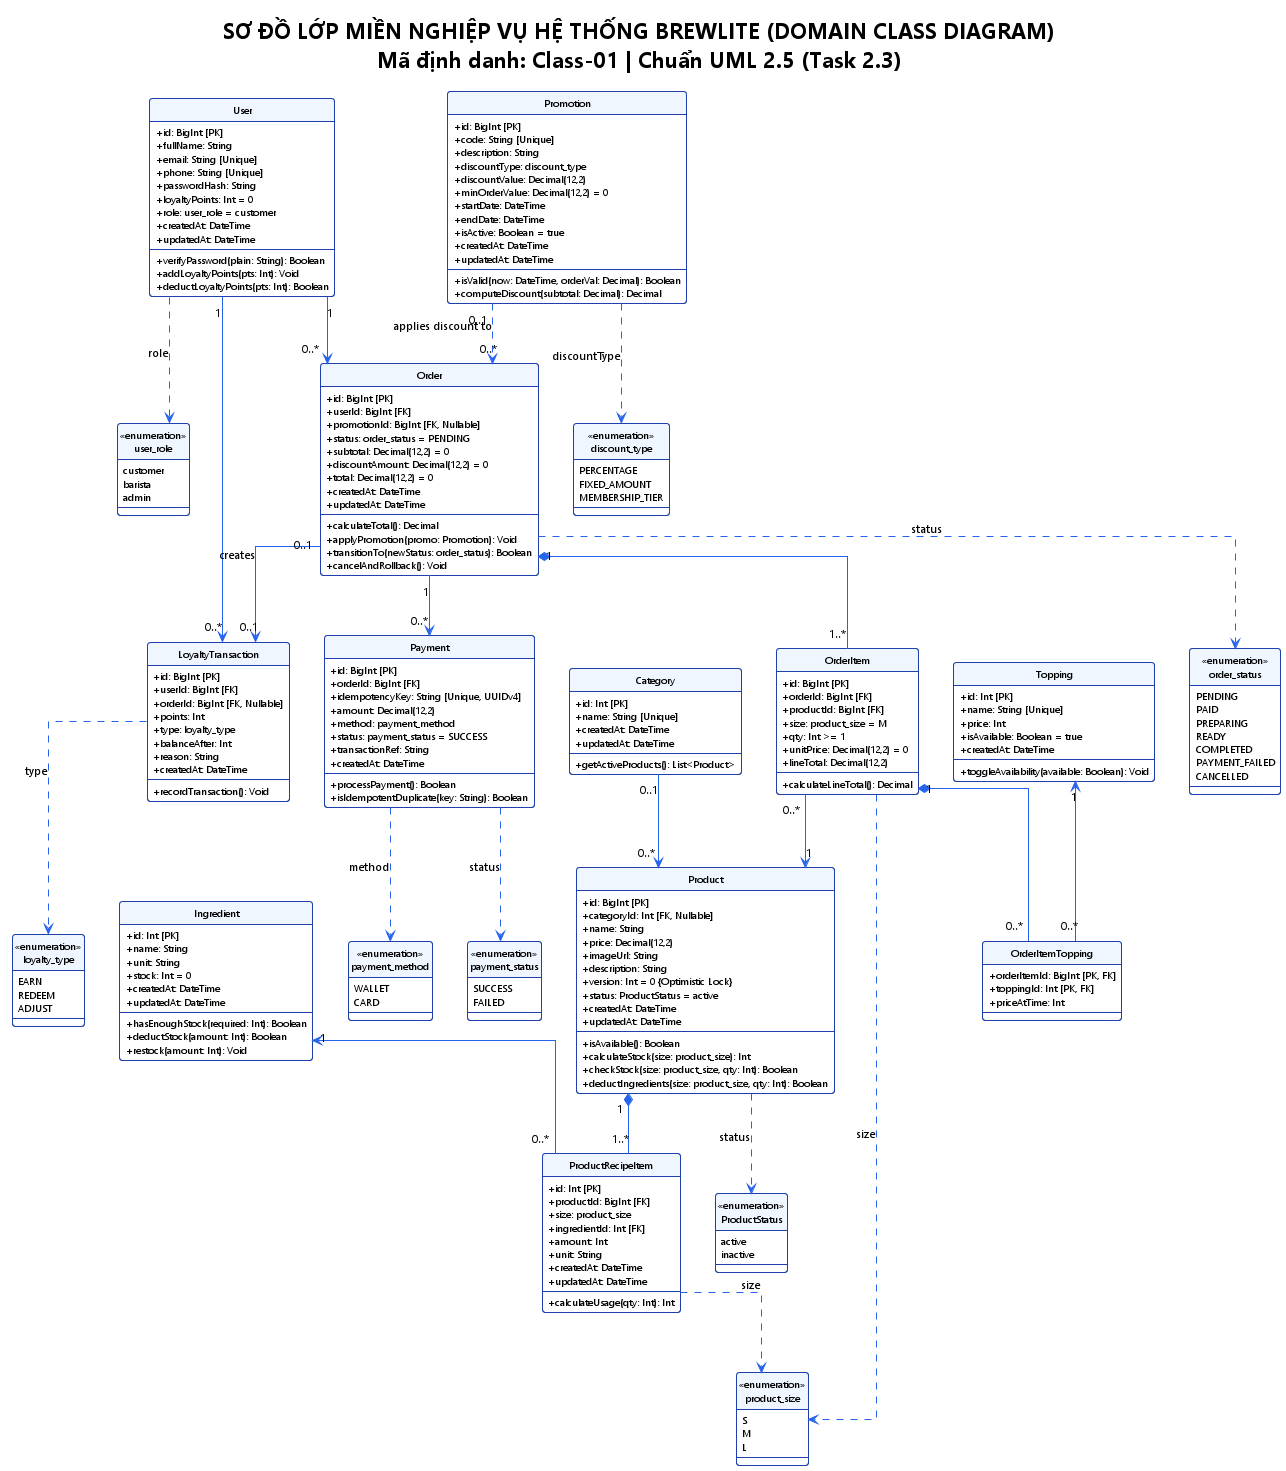
\includegraphics[width=\textwidth]{class-diagram.png}
    }{%
        \fbox{\begin{minipage}{0.95\textwidth}
            \centering
            \vspace{0.5cm}
            \textbf{Sơ đồ Lớp Miền Nghiệp Vụ BrewLite (Class-01)}\\[0.2cm]
            \textit{(Tệp đồ họa vector sắc nét lưu tại: \texttt{docs/diagrams/class-diagram.svg})}\\[0.2cm]
            Mô hình hóa 12 thực thể miền, 8 Enumerations trạng thái, cùng các quan hệ Composition và Association hoàn chỉnh.
            \vspace{0.5cm}
        \end{minipage}}
    }
    \caption{Sơ đồ Lớp Miền Nghiệp Vụ Hệ Thống BrewLite (UML 2.5)}
    \label{fig:class-diagram}
\end{figure}

\section{Đặc tả chi tiết các Lớp Miền Nghiệp Vụ (Domain Entities)}

Hệ thống bao gồm \textbf{12 thực thể} (đáp ứng trọn vẹn 7 thực thể bắt buộc của đề bài cùng 5 thực thể quản lý phân loại danh mục, topping, nguyên vật liệu và công thức định mức pha chế):

\vspace{0.2cm}
\noindent
\footnotesize
\renewcommand{\arraystretch}{1.25}
\begin{xltabular}{\textwidth}{|c|>{\raggedright\arraybackslash}p{3.2cm}|>{\raggedright\arraybackslash}p{4.2cm}|>{\raggedright\arraybackslash}X|}
\caption{Danh mục 12 Lớp Miền Nghiệp Vụ trong Hệ Thống} \label{tab:classes} \\
\hline
\rowcolor{tableheader}
\textbf{STT} & \textbf{Tên Lớp} & \textbf{Thuộc tính chính \& Kiểu dữ liệu} & \textbf{Phương thức nghiệp vụ chính} \\
\hline
\endfirsthead

\hline
\rowcolor{tableheader}
\textbf{STT} & \textbf{Tên Lớp} & \textbf{Thuộc tính chính \& Kiểu dữ liệu} & \textbf{Phương thức nghiệp vụ (tiếp theo)} \\
\hline
\endhead

\hline
\endfoot

\hline
\endlastfoot

\textbf{1} & \textbf{User}\newline\textit{(Bắt buộc)} & 
\texttt{id: BigInt [PK]}\newline
\texttt{fullName: String}\newline
\texttt{email: String [Unique]}\newline
\texttt{phone: String [Unique]}\newline
\texttt{passwordHash: String}\newline
\texttt{loyaltyPoints: Int = 0}\newline
\texttt{role: user\_role = customer}\newline
\texttt{createdAt, updatedAt: DateTime} & 
\texttt{verifyPassword(plain): Boolean}\newline
\texttt{addLoyaltyPoints(pts): Void}\newline
\texttt{deductLoyaltyPoints(pts): Boolean}\newline
Quản lý tài khoản người dùng, mã hóa mật khẩu \texttt{bcrypt}, phân quyền (customer, barista, admin) và tích lũy điểm thưởng. \\
\hline

\textbf{2} & \textbf{Product}\newline\textit{(Bắt buộc)} & 
\texttt{id: BigInt [PK]}\newline
\texttt{categoryId: Int [FK, Null]}\newline
\texttt{name: String}\newline
\texttt{price: Decimal(12,2)}\newline
\texttt{imageUrl, description: String}\newline
\texttt{version: Int = 0 \{Lock\}}\newline
\texttt{status: ProductStatus = active}\newline
\texttt{createdAt, updatedAt: DateTime} & 
\texttt{isAvailable(): Boolean}\newline
\texttt{calculateStock(size): Int}\newline
\texttt{checkStock(size, qty): Boolean}\newline
\texttt{deductIngredients(size, qty): Boolean}\newline
Quản lý thông tin đồ uống; tính tồn kho khả dụng tự động qua công thức và trừ kho nguyên liệu; kiểm soát khóa lạc quan qua \texttt{version}. \\
\hline

\textbf{3} & \textbf{Order}\newline\textit{(Bắt buộc)} & 
\texttt{id: BigInt [PK]}\newline
\texttt{userId: BigInt [FK]}\newline
\texttt{promotionId: BigInt [FK, Null]}\newline
\texttt{status: order\_status = PENDING}\newline
\texttt{subtotal: Decimal(12,2) = 0}\newline
\texttt{discountAmount: Decimal = 0}\newline
\texttt{total: Decimal(12,2) = 0}\newline
\texttt{createdAt, updatedAt: DateTime} & 
\texttt{calculateTotal(): Decimal}\newline
\texttt{applyPromotion(promo): Void}\newline
\texttt{transitionTo(newStatus): Boolean}\newline
\texttt{cancelAndRollback(): Void}\newline
Thực thi máy trạng thái 7 bước, tính toán giảm giá voucher, tổng tiền đơn và hoàn trả nguyên vật liệu nếu hủy đơn. \\
\hline

\textbf{4} & \textbf{OrderItem}\newline\textit{(Bắt buộc)} & 
\texttt{id: BigInt [PK]}\newline
\texttt{orderId: BigInt [FK]}\newline
\texttt{productId: BigInt [FK]}\newline
\texttt{size: product\_size = M}\newline
\texttt{qty: Int >= 1}\newline
\texttt{unitPrice: Decimal(12,2)}\newline
\texttt{lineTotal: Decimal(12,2)} & 
\texttt{calculateLineTotal(): Decimal}\newline
Từng dòng món đặt trong đơn hàng kèm cấu hình dung tích kích cỡ (S, M, L), đơn giá và thành tiền tương ứng. \\
\hline

\textbf{5} & \textbf{Payment}\newline\textit{(Bắt buộc)} & 
\texttt{id: BigInt [PK]}\newline
\texttt{orderId: BigInt [FK]}\newline
\texttt{idempotencyKey: String [Unique]}\newline
\texttt{amount: Decimal(12,2)}\newline
\texttt{method: payment\_method}\newline
\texttt{status: payment\_status = SUCCESS}\newline
\texttt{transactionRef: String}\newline
\texttt{createdAt: DateTime} & 
\texttt{processPayment(): Boolean}\newline
\texttt{isIdempotentDuplicate(key): Boolean}\newline
Xử lý giao dịch thanh toán trực tuyến (Ví điện tử hoặc Thẻ), chống trừ tiền trùng lặp bằng khóa duy nhất Idempotency Key. \\
\hline

\textbf{6} & \textbf{Promotion}\newline\textit{(Bắt buộc)} & 
\texttt{id: BigInt [PK]}\newline
\texttt{code: String [Unique]}\newline
\texttt{description: String}\newline
\texttt{discountType: discount\_type}\newline
\texttt{discountValue, minOrderValue}\newline
\texttt{startDate, endDate: DateTime}\newline
\texttt{isActive: Boolean = true}\newline
\texttt{createdAt, updatedAt: DateTime} & 
\texttt{isValid(now, orderVal): Boolean}\newline
\texttt{computeDiscount(subtotal): Decimal}\newline
Quản lý mã giảm giá, voucher khuyến mãi và chiết khấu ưu đãi theo hạn mức và thời gian hiệu lực. \\
\hline

\textbf{7} & \textbf{LoyaltyTransaction}\newline\textit{(Bắt buộc)} & 
\texttt{id: BigInt [PK]}\newline
\texttt{userId: BigInt [FK]}\newline
\texttt{orderId: BigInt [FK, Nullable]}\newline
\texttt{points: Int}\newline
\texttt{type: loyalty\_type}\newline
\texttt{balanceAfter: Int}\newline
\texttt{reason: String}\newline
\texttt{createdAt: DateTime} & 
\texttt{recordTransaction(): Void}\newline
Lưu vết chi tiết lịch sử cộng/trừ điểm thưởng thành viên (tỷ lệ $10.000$đ = 1 điểm khi hoàn tất đơn hàng). \\
\hline

\textbf{8} & \textbf{Ingredient} & 
\texttt{id: Int [PK]}\newline
\texttt{name: String}\newline
\texttt{unit: String}\newline
\texttt{stock: Int = 0}\newline
\texttt{createdAt, updatedAt: DateTime} & 
\texttt{hasEnoughStock(req): Boolean}\newline
\texttt{deductStock(amount): Boolean}\newline
\texttt{restock(amount): Void}\newline
Quản lý định lượng nguyên vật liệu lưu kho (cà phê Robusta/Arabica, sữa đặc, sữa tươi, siro, trà đen,...). \\
\hline

\textbf{9} & \textbf{ProductRecipeItem} & 
\texttt{id: Int [PK]}\newline
\texttt{productId: BigInt [FK]}\newline
\texttt{size: product\_size}\newline
\texttt{ingredientId: Int [FK]}\newline
\texttt{amount: Int}\newline
\texttt{unit: String}\newline
\texttt{createdAt, updatedAt: DateTime} & 
\texttt{calculateUsage(qty): Int}\newline
Bảng định lượng công thức pha chế (BOM) chi tiết cho từng loại đồ uống theo từng kích cỡ ly. \\
\hline

\textbf{10} & \textbf{Category} & 
\texttt{id: Int [PK]}\newline
\texttt{name: String [Unique]}\newline
\texttt{createdAt, updatedAt: DateTime} & 
\texttt{getActiveProducts(): List<Product>}\newline
Phân nhóm thực đơn (Cà phê, Trà trái cây, Trà sữa, Đá xay \& Thức uống khác). \\
\hline

\textbf{11} & \textbf{Topping} & 
\texttt{id: Int [PK]}\newline
\texttt{name: String [Unique]}\newline
\texttt{price: Int}\newline
\texttt{isAvailable: Boolean = true}\newline
\texttt{createdAt: DateTime} & 
\texttt{toggleAvailability(status): Void}\newline
Món dùng kèm (trân châu, kem cheese, thạch dừa). \\
\hline

\textbf{12} & \textbf{OrderItemTopping} & 
\texttt{orderItemId: BigInt [PK, FK]}\newline
\texttt{toppingId: Int [PK, FK]}\newline
\texttt{priceAtTime: Int} & 
Liên kết trung gian lưu vết giá topping tại thời điểm khách đặt hàng (\texttt{onDelete: Cascade}). \\
\hline
\end{xltabular}

\section{Các kiểu Liệt kê Trạng thái \& Nghiệp vụ (Enumerations)}

\vspace{0.2cm}
\noindent
\small
\renewcommand{\arraystretch}{1.3}
\begin{xltabular}{\textwidth}{|c|>{\raggedright\arraybackslash}p{3cm}|>{\raggedright\arraybackslash}p{4.2cm}|>{\raggedright\arraybackslash}X|}
\caption{Danh mục 8 Kiểu Liệt Kê Chuẩn Hóa Theo CSDL} \label{tab:enums} \\
\hline
\rowcolor{tableheader}
\textbf{STT} & \textbf{Tên Enum} & \textbf{Các giá trị hợp lệ} & \textbf{Ý nghĩa \& Nguồn kiểm chứng} \\
\hline
\endfirsthead

\hline
\rowcolor{tableheader}
\textbf{STT} & \textbf{Tên Enum} & \textbf{Các giá trị hợp lệ} & \textbf{Ý nghĩa (tiếp theo)} \\
\hline
\endhead

\hline
\endfoot

\hline
\endlastfoot

\textbf{1} & \texttt{user\_role} & \texttt{customer}, \texttt{barista}, \texttt{admin} & Phân quyền truy cập người dùng trong hệ thống (RBAC) theo \texttt{schema.prisma}. \\
\hline
\textbf{2} & \texttt{order\_status} & \texttt{PENDING}, \texttt{PAID}, \texttt{PREPARING}, \texttt{READY}, \texttt{COMPLETED}, \texttt{PAYMENT\_FAILED}, \texttt{CANCELLED} & Vòng đời 7 trạng thái của đơn hàng theo máy trạng thái hữu hạn FSM. \\
\hline
\textbf{3} & \texttt{payment\_method} & \texttt{WALLET}, \texttt{CARD} & Phương thức thanh toán mô phỏng (Ví điện tử hoặc Thẻ). \\
\hline
\textbf{4} & \texttt{payment\_status} & \texttt{SUCCESS}, \texttt{FAILED} & Trạng thái ghi nhận kết quả xử lý giao dịch thanh toán. \\
\hline
\textbf{5} & \texttt{product\_size} & \texttt{S}, \texttt{M}, \texttt{L} & Kích cỡ đồ uống (Size S cơ sở, M $+5.000$đ, L $+10.000$đ). \\
\hline
\textbf{6} & \texttt{ProductStatus} & \texttt{active}, \texttt{inactive} & Trạng thái kinh doanh bật/tắt của món đồ uống. \\
\hline
\textbf{7} & \texttt{discount\_type} & \texttt{PERCENTAGE}, \texttt{FIXED\_AMOUNT}, \texttt{MEMBERSHIP\_TIER} & Phân loại hình thức chiết khấu khuyến mãi (Domain). \\
\hline
\textbf{8} & \texttt{loyalty\_type} & \texttt{EARN}, \texttt{REDEEM}, \texttt{ADJUST} & Bản chất giao dịch điểm thưởng (Tích điểm khi đơn PAID, Đổi điểm thưởng, Điều chỉnh). \\
\hline
\end{xltabular}

\section{Quan hệ \& Ràng buộc Đa số (Multiplicity)}

Các mối quan hệ cấu trúc tuân thủ nghiêm ngặt ngữ nghĩa UML 2.5:

\begin{itemize}[leftmargin=*,itemsep=3pt]
    \item \textbf{\texttt{Category} $0..1$ -- $0..*$ \texttt{Product} (Association):} Một sản phẩm có thể thuộc về $0$ hoặc $1$ danh mục (\texttt{categoryId} nullable). Một danh mục chứa từ $0$ đến nhiều sản phẩm.
    \item \textbf{\texttt{Product} $1$ *-- $1..*$ \texttt{ProductRecipeItem} (Composition):} Mỗi sản phẩm bao gồm một hoặc nhiều định lượng công thức pha chế theo từng size. Khi xóa sản phẩm, các công thức con tự động bị xóa theo (\texttt{onDelete: Cascade}).
    \item \textbf{\texttt{Ingredient} $1$ <-- $0..*$ \texttt{ProductRecipeItem} (Association):} Một nguyên vật liệu lưu kho có thể được sử dụng trong công thức của nhiều sản phẩm khác nhau.
    \item \textbf{\texttt{OrderItem} $0..*$ -- $1$ \texttt{Product} (Association):} Mỗi dòng chi tiết đơn hàng tham chiếu đến duy nhất 1 sản phẩm xác định.
    \item \textbf{\texttt{User} $1$ -- $0..*$ \texttt{Order} (Association):} Một khách hàng có thể khởi tạo $0$ hoặc nhiều đơn hàng.
    \item \textbf{\texttt{Order} $1$ *-- $1..*$ \texttt{OrderItem} (Composition -- Hợp thành sống còn):} Mỗi đơn hàng bắt buộc phải có từ 1 đến nhiều món. Khi đơn hàng bị xóa khỏi hệ thống, các \texttt{OrderItem} con tự động bị xóa theo (\texttt{onDelete: Cascade}).
    \item \textbf{\texttt{OrderItem} $1$ *-- $0..*$ \texttt{OrderItemTopping} (Composition):} Mỗi món đồ uống có thể chọn từ 0 đến nhiều loại topping đi kèm (\texttt{onDelete: Cascade}).
    \item \textbf{\texttt{Topping} $1$ <-- $0..*$ \texttt{OrderItemTopping} (Association):} Một loại topping có thể được chọn trong nhiều mục đặt hàng.
    \item \textbf{\texttt{Order} $1$ -- $0..*$ \texttt{Payment} (Association):} Một đơn hàng liên kết với các lượt thanh toán qua khóa ngoại \texttt{orderId}. Cho phép ghi nhận các lần thanh toán thất bại trước khi thanh toán thành công.
    \item \textbf{\texttt{Promotion} $0..1$ ..> $0..*$ \texttt{Order} (Dependency):} Một đơn hàng có thể không áp dụng hoặc áp dụng tối đa một mã ưu đãi/chiết khấu thành viên (\texttt{promotionId} nullable).
    \item \textbf{\texttt{User} $1$ -- $0..*$ \texttt{LoyaltyTransaction} (Association):} Một tài khoản khách hàng sở hữu toàn bộ lịch sử các giao dịch điểm tích lũy.
    \item \textbf{\texttt{Order} $0..1$ -- $0..1$ \texttt{LoyaltyTransaction} (Association):} Mỗi đơn hàng thanh toán thành công (\texttt{PAID}) phát sinh duy nhất một giao dịch cộng điểm thưởng ($10.000\text{đ} = 1\text{ điểm}$).
\end{itemize}

\section{Chứng minh Tiêu chí Nghiệm thu Khắt khe (Zero Contradiction)}

\vspace{0.2cm}
\noindent
\footnotesize
\renewcommand{\arraystretch}{1.25}
\begin{xltabular}{\textwidth}{|c|>{\raggedright\arraybackslash}p{3.8cm}|>{\raggedright\arraybackslash}p{3.8cm}|>{\raggedright\arraybackslash}X|}
\caption{Bảng Đối Chiếu Tính Nhất Quán Tuyệt Đối Của Sơ Đồ Lớp} \label{tab:consistency} \\
\hline
\rowcolor{tableheader}
\textbf{STT} & \textbf{Tài liệu đối chiếu} & \textbf{Điểm ràng buộc kỹ thuật} & \textbf{Minh chứng tính nhất quán trong Class Diagram} \\
\hline
\endfirsthead

\hline
\rowcolor{tableheader}
\textbf{STT} & \textbf{Tài liệu đối chiếu} & \textbf{Điểm ràng buộc kỹ thuật} & \textbf{Minh chứng (tiếp theo)} \\
\hline
\endhead

\hline
\endfoot

\hline
\endlastfoot

\textbf{1} & \textbf{Cơ sở dữ liệu \& Seed}\newline\path{apps/api/prisma/schema.prisma}\newline\path{brewlite_seed_data.sql} & Khóa chính, khóa ngoại, kiểu dữ liệu, enum vai trò, tồn kho theo nguyên liệu, bảng thanh toán. & 
Trùng khớp 100\% các kiểu: \texttt{BigInt}, \texttt{Decimal(12,2)}, \texttt{DateTime}.\newline
Trường \texttt{Product.version} thực thi Optimistic Concurrency Control.\newline
Trừ kho theo nguyên liệu qua \texttt{Ingredient} và \texttt{ProductRecipeItem}.\newline
Trường \texttt{Payment.idempotencyKey} gán thuộc tính \texttt{[Unique]}.\newline
Đầy đủ 3 vai trò \texttt{user\_role} (\texttt{customer}, \texttt{barista}, \texttt{admin}).\newline
Bảng \texttt{Payment} có \texttt{status} và \texttt{transactionRef}. \\
\hline

\textbf{2} & \textbf{Đặc tả yêu cầu (SRS)}\newline\path{srs.md} & Các mã chức năng: FR-01, FR-02, FR-03, FR-05, FR-06, FR-07, FR-08, FR-11. & 
FR-01/02 qua \texttt{Product}, \texttt{Category}, \texttt{Ingredient}, \texttt{Topping}.\newline
FR-03 qua \texttt{OrderItem} và \texttt{OrderItemTopping}.\newline
FR-05 qua \texttt{Order.status = PENDING}.\newline
FR-06 qua \texttt{Payment.idempotencyKey}.\newline
FR-07/11 qua \texttt{LoyaltyTransaction} và \texttt{Promotion}.\newline
FR-08 qua \texttt{order\_status} FSM. \\
\hline

\textbf{3} & \textbf{Sơ đồ tuần tự}\newline\path{sequence-checkout.puml} & Thứ tự gọi hàm, transaction tạo đơn và xác thực thanh toán qua cổng mô phỏng. & 
Khớp chính xác các tham số gọi trong Sequence: hàm tạo đơn \texttt{POST /orders} tạo đối tượng \texttt{Order} \& \texttt{OrderItem}; hàm \texttt{POST /payments} kiểm tra trùng \texttt{idempotencyKey} và nạp giao dịch \texttt{LoyaltyTransaction}. \\
\hline

\textbf{4} & \textbf{Sơ đồ hoạt động}\newline\path{activity-order-flow.puml} & Nhánh kiểm tra tồn kho nguyên liệu, nhánh hủy đơn và rollback khi thanh toán lỗi. & 
Nhánh kiểm tra tồn kho khớp với \texttt{Product.checkStock()} và \texttt{Ingredient.hasEnoughStock()}.\newline
Nhánh hủy đơn quá hạn/thanh toán thất bại khớp với phương thức \texttt{Order.cancelAndRollback()} hoàn lại nguyên liệu. \\
\hline
\end{xltabular}

\end{document}
